\chapter{TemplateFactory}
Creates Javascript function templates from a given ROOT class using \textit{TClassRef}. Methods and static members are set during creation through the use of ROOT reflections and the proxy factories. 
The created templates are kept in a cache to avoid unnecessary creation of already existing templates.
\section{createTemplate}
\begin{longtable}{p{3cm} @{\hskip 1cm} p{12cm}}
 \hline
\textit{Name} & \texttt{TemplateFactory::createTemplate(clazz: TClassRef)}\\
\hline
 \textit{Visibility} & public\\
\hline
\textit{Parameters} & \textit{clazz: TClassRef} the class for which a template is to be created \\
\hline
\textit{Return value} & \textbf{ Local<FunctionTemplate>} the created template\\
  \hline
 \textit{Behavior} & Gets the class from TClassRef and creates a new function template. 
			Then it iterates over all static members of the class and sets the
			corresponding members of the template to respective proxy objects.
			It then iterates through the functions and also sets them.
			For further reference consider the following sequence diagram.\\
\hline
\end{longtable} \pagebreak
 
\begin{figure}[htb]
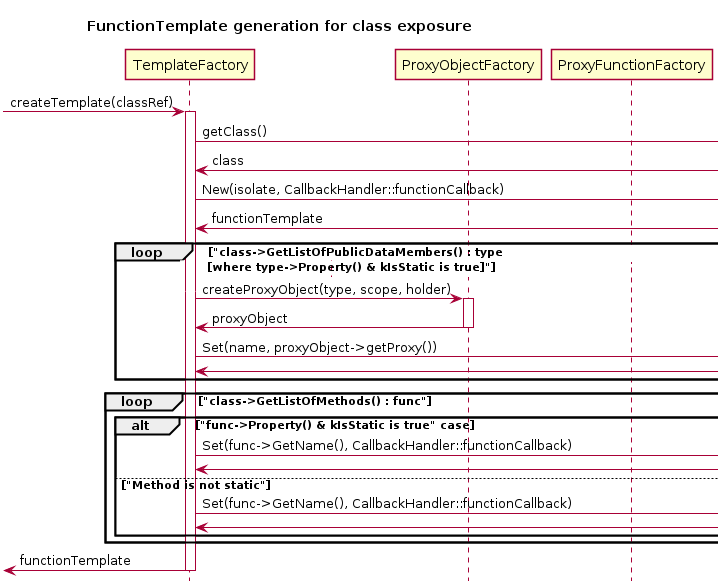
\includegraphics[width=16cm]{./latex/resources/functionTemplateGenerateCrop.png}
	\caption{function template creation (full diagram in appendix)}
\end{figure}
